\documentclass[tikz,border=4pt]{standalone}
\usetikzlibrary{positioning, fit, backgrounds, arrows.meta}

\tikzset{
  stage/.style       = {draw, thick, rounded corners=2pt, fill=white,
                        minimum width=21mm, minimum height=11mm, align=center},
  data/.style        = {stage, fill=gray!12},
  block/.style       = {draw=blue!50, fill=blue!6, rounded corners=4pt, inner sep=3mm},
  block title/.style = {font=\bfseries\small, text=blue!50!black},
  >={Stealth[length=2.5mm]},
}

\begin{document}
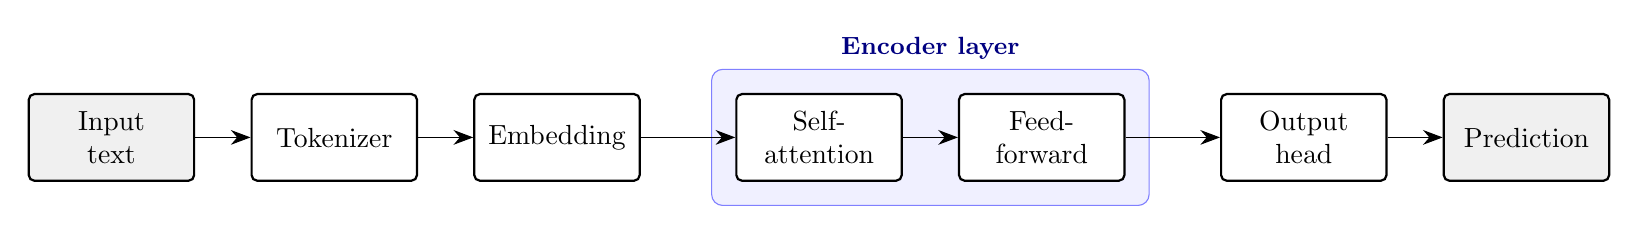
\begin{tikzpicture}[node distance=6mm and 7mm]
  \node[data]                     (input) {Input\\ text};
  \node[stage]    (tok) at (2.83,0)   {Tokenizer};
  \node[stage, right=3.53cm of input]      (embed) {Embedding};
  \node[stage, right=12mm of embed] (attn) {Self-\\ attention};
  \node[stage, right=of attn]     (ffn)   {Feed-\\ forward};
  \node[stage, right=12mm of ffn] (head)  {Output\\ head};
  \node[data, right=of head]      (out)   {Prediction};

  \draw[->] (input) -- (tok);
  \draw[->] (tok)   -- (embed);
  \draw[->] (embed) -- (attn);
  \draw[->] (attn)  -- (ffn);
  \draw[->] (ffn)   -- (head);
  \draw[->] (head)  -- (out);

  \begin{scope}[on background layer]
    \node[block, fit=(attn) (ffn), label={[block title]north:Encoder layer}] (encoder) {};
  \end{scope}
\end{tikzpicture}
\end{document}
